\section{Patterns}
\label{sec:patterns}

Using software design patterns can provide some consistency and structure throughout an application. Using the tools that Android provides, one will automatically use certain patterns. These are described below, along with the patterns that was found relevant for this project.

\paragraph{Model-View-Controller}
Android programming is built around a large toolbox which provides many shortcuts to achieve a nice looking application easily. An important basic element is the 'Activity' which enables the creation of a graphical window for the user. An Activity consists of a Java file and an XML file. The latter describes the layout that should be shown on screen. Through the Java file, one indicates that the XML file should be used as layout, and behavior can then be implemented for what should happen when the user presses a button, slides the screen or any other event that might occur. These activities have life-cycles as seen in \ref{fig:lifecycle}. This allows the specification of what should happen on each change in the life-cycle. For example on creation of the activity (onCreate), or when it becomes obscured by another element (onPause) such as a dialog box or another Activity.

This Activity-structure implicates an implementation of Model-View-Controller as a pattern where the view is created through XML. The Java file then acts as a controller for the View. The model however is not included as part as the Activity; this is up to the developer to implement. One can argue that Model-View-Presenter, a derivative of MVC, is even more applicable. This would describe the Java-file of the Activity as a presenter rather than controller. This fits from the perspective that it does not by default specify which views are displayed, and that the views themselves contain little to no logic. This is all handled by the presenter. There is however flaws to this as well. Layout files can for example have selectors which contains logic describing a view depending on a state. (Hence, the view is not stateless as described by MVP).

The feature set of Android does not match either MVC or MVP perfectly, and for this project, using Android features extensively, the pattern used is a mixture of the two. For a comparison between the two patterns, see \citep{MVC_MVP}

\paragraph{Composite}
Another pattern encountered with Android is the Composite pattern. The XML-files containing layouts will often be composites. This happens because elements such as buttons, sliders, views and other components usually are grouped within layouts such as RelativeLayout or LinearLayout. For example, a RelativeLayout could be composed by an ImageView, TextView and two RadioButton. Using this pattern is not without reason, as it enables the manipulation of entire composite layouts, rather than individual objects. An example could be to give a certain layout a background color, spanning between all the components within that layout.

\paragraph{Adapter}
The Adapter pattern is used in the standard implementation of views containing lists in Android. Say for example that one wants to display a list of persons in an Activity, one would have to figure out how many views to create, how to display the data, and how to update it if a person is added or removed. Android uses an array of different adapters to assist on this. By default, the developer only has to create a single view for one element, or per example, person. The adapter can then, given a list of elements, handle the creation and destruction of views needed to display this list.

\paragraph{Facade}
The Facade pattern is not related to Android. It is used for hiding away ugly logics that the developer does not need to know the details about, in order to use them. In this project, the application needs to communicate with a server. The pattern is chosen because it would be messy to implement the communication directly in each Activity. Instead, this should be hidden somewhere else, providing only a "Facade" to use in the Activities. This way the programmer only has to worry about what to send to a server, rather than having to package it properly, deal with threading for network communication, or disassembling responses from the server.

\begin{figure}[H]
	\centering
	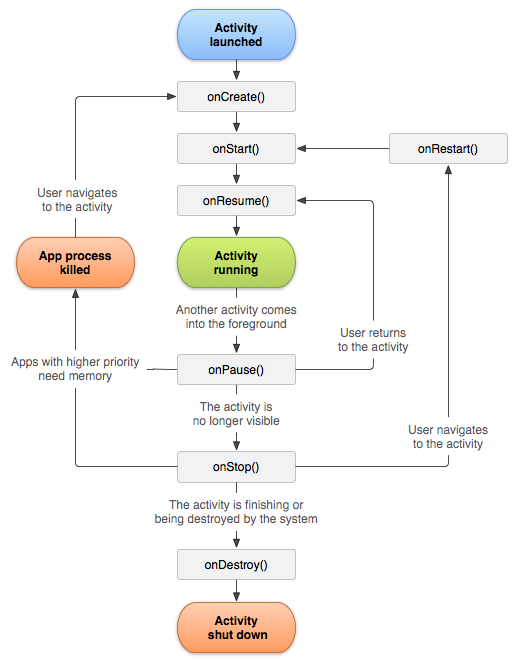
\includegraphics[width=\textwidth]{Pictures/activity_lifecycle.png}
	\caption{Lifecycle of an Android Activity}
	\label{fig:lifecycle}
\end{figure}